% !TEX root = ../report.tex
\section{Постановка задачи}

\subsection{Индивидуальное задание}

\textbf{Вариант 10, OpenMP.}

Определить частоту встречи слов в тексте на русском языке.

\subsection{Программа работы}

\begin{enumerate}
\item Для алгоритма из полученного задания написать последовательную программу на языке C или С++, реализующую этот алгоритм.
\item Для созданной последовательной программы необходимо написать 3-5 тестов, которые покрывают основные варианты функционирования программы. Для создания тестов можно воспользоваться механизмом Unit-тестов среды NetBeans, или описать входные тестовые данные в файлах. При использовании NetBeans необходимо в свойствах проекта установить ключ компилятора -pthread.
\item Проанализировать полученный алгоритм, выделить части, которые могут быть распараллелены, разработать структуру параллельной программы. Определить количество используемых потоков, а также правила и используемые объекты синхронизации.
\item Согласовать разработанную структуру и детали реализации параллельной программы с преподавателем.
\item Написать код параллельной программы и проверить ее корректность на созданном ранее наборе тестов. При необходимости найти и исправить ошибки.
\item Провести эксперименты для оценки времени выполнения последовательной и параллельной программ. Проанализировать полученные результаты.
\item Сделать общие выводы по результатам проделанной работы: 
\begin{itemize}
\item Различия между способами проектирования последовательной и параллельной реализаций алгоритма.
\item Возможные способы выделения параллельно выполняющихся частей, Возможные правила синхронизации потоков.
\item Сравнение времени выполнения последовательной и параллельной программ.
\item Принципиальные ограничения повышения эффективности параллельной реализации по сравнению с последовательной.
\end{itemize}
\end{enumerate}

\section{Сведения о системе}
Работа производилась на реальной системе, со следующими характеристиками:

\begin{table}[H]
	\centering
	\begin{tabular}{|M{5cm}|M{10cm}|}
		\hline ОС & Windows 10 Домашняя для одного языка     \\
		\hline Версия     & Версия 1709 (Сборка ОС 16299.431)  \\
		\hline Установленная оперативная память (RAM)     & 8 ГБ     \\
		\hline Процессор     & Intel(R) Core(TM) i7-3537U CPU @ 2.00 GHz 2.50 GHz, ядер: 2, логических процессоров: 4   \\
		\hline		
	\end{tabular}
	\caption{Сведения о системе}
	\label{tab:task}
\end{table}

\section{Структура проекта}

\begin{figure}[H]
	\centering
	\framebox[\textwidth]{%
		\begin{minipage}{\textwidth}
			\dirtree{%
				.1 project.
				.2 source code.
				.3 main.cpp.
				.3 utils.cpp.
				.2 header files.
				.3 utils.h.
			}
		\end{minipage}
	}
\caption{Структура проекта}
\end{figure}

Точка входа расположена в файле \textbf{main.cpp}, в котором вызываются необходимые функции, реализованные в \textbf{utils.cpp}.

Текст для анализа загружается из файла построчно и хранится в переменной типа string.

Итоговый список встреченных слов в тексте представлен в виде unordered\_map<string, int> со словом в качестве ключа и количеством встреч в тексте в качестве значения.

Стоит обратить внимание на функцию \texttt{getStringPart()} в файле \textbf{utils.cpp}, которая позволяет скорректировать подстроку таким образом, чтобы в ее конце не оказалось обрезанного слова и разделителей, а в начале разделителей. Для ее корректной работы необходимо, чтобы подстрока начиналась с начала слова либо разделителя. Таким образом, при исполнении в цикле для следующей подстроки в качестве стартового индекса используется конечный индекс предыдущей подстроки, полученный при использовании функции.

Функция \texttt{getCutIndex()} используется в качестве псевдонима функций find\_* для большей читаемости кода.

\lstset{style=C++}
\begin{lstlisting}[label=lst:VHDL,caption=отрывок utils.cpp]
// beginInd must be at word start or delimiter
std::pair<int, int> getStringPart(const std::string &str, unsigned int beginInd, unsigned int endInd) {
	std::pair<int, int> ind;

	// cut delimiter if needed from start
	ind.first = (getCutIndex(str, beginInd, WORD_0) == beginInd) ? getCutIndex(str, beginInd, SPACE_0) : beginInd;
	// cut delimiter if needed or restore cut word from end
	ind.second = (getCutIndex(str, endInd, WORD_N) == endInd) ? getCutIndex(str, endInd, SPACE_N) : getCutIndex(str, endInd, WORD_0) - 1;

	return ind;	
}

unsigned int getCutIndex(const std::string &str, int pos, cutType type) {
	std::string delim = " .,!?&@():;-|\"\r\n";
	switch(type) {
		case(SPACE_0):
			return str.find_first_not_of(delim, pos);
		case(SPACE_N):
			return str.find_last_not_of(delim, pos);
		case(WORD_0):
			return str.find_first_of(delim, pos);
		case(WORD_N):
			return str.find_last_of(delim, pos);
		default:
			return -1;
	}
}
\end{lstlisting}

Полный исходный код приведен в листинге \vref{lst:utilscpp}.

\section{Алгоритм решения}

\subsection{Последовательная реализация}

Алгоритм заключается в вызове функции \texttt{getWordDict()}, которая проходит по строке, находит слова и формирует unordered\_map.

\begin{lstlisting}[label=lst:VHDL,caption=отрывок utils.cpp]
std::unordered_map<std::string, int> getWordDict(const std::string &str, unsigned int strBegin, unsigned int strEnd) {
	std::unordered_map<std::string, int> dict;

	while((strBegin = getCutIndex(str, strBegin, SPACE_0)) < strEnd){
		int cutEnd = getCutIndex(str, strBegin, WORD_0);
		int strLength = cutEnd - strBegin;
		std::string temp = str.substr(strBegin, strLength);

		strBegin = getCutIndex(str, cutEnd, SPACE_0);
		dict[temp] += 1;
	}

	return dict;
}
\end{lstlisting}

\subsection{Параллельная реализация с использованием pthreads}

В отличии от последовательной реализации, в данном случае накладывается ограничение на количество возможных потоков.

Общий алгоритм остается тем же, но перед запуском потоков исходная строка разбивается на число подстрок равное числу потоков и корректируются функцией \texttt{getStringPart()}, чтобы в подстроках не было обрезанных слов либо слов, попавших в обе подстроки. Затем, после получения массива unordered\_map, происходит их слияние в одном потоке (функция \texttt{mergeDict()} в листинге \vref{lst:utilscpp}).

\begin{lstlisting}[label=lst:VHDL,caption=отрывок utils.cpp]
void *getWordDict_pthread(void *args) {
	getWordDictArgs *arg = (getWordDictArgs *)args; 
	std::unordered_map<std::string, int> dict;

	if(!arg->str.empty()) {
		while((arg->strBegin = getCutIndex(arg->str, arg->strBegin, SPACE_0)) < arg->strEnd){
			int cutEnd = getCutIndex(arg->str, arg->strBegin, WORD_0);
			int strLength = cutEnd - arg->strBegin;
			std::string temp = arg->str.substr(arg->strBegin, strLength);

			arg->strBegin = getCutIndex(arg->str, cutEnd, SPACE_0);
			dict[temp] += 1;
		}
	}

	arg->dict = dict;
	return 0;
}
\end{lstlisting}

\subsection{Параллельная реализация с использованием OpenMP}

Алгоритм для OpenMP аналогичен Pthreads. Благодаря использованию директив, удалось сильно сократить количество строк реализации.

В данном случае, была использована директива \texttt{\#pragma omp parallel for} для параллельного вызова функции \texttt{getWordDict()}.

\begin{lstlisting}[label=lst:VHDL,caption=отрывок main.cpp]
omp_set_num_threads(threadCount);
#pragma omp parallel for
	for(int i = 0; i < threadCount; i++) {
		dicts[i] = getWordDict(args[i].str, args[i].strBegin, args[i].strEnd);
	}
\end{lstlisting}

Полный исходный код приведен в листинге \vref{lst:main}.

\section{Тестирование}

В качестве исходного теста использовалась книга "`Гарри Поттер и Орден Феникса"', увеличение текста производилось удвоением содержимого.

\subsection{Эксперимент 1}

\textbf{Количество потоков}: 4 (равно числу логических процессоров)

\textbf{Количество слов в тексте}: 269374 -- 8619968

\begin{table}[H]
	\centering
	\begin{tabular}{|c|c|c|c|}
		\hline
		Число слов в тексте        & Последовательный & OpenMP & Pthreads \\ \hline
		269374  & 0.403            & \textbf{0.206} & 0.226 \\ \hline
		538748  & 0.813            & 0.433 & \textbf{0.429} \\ \hline
		1077496 & 1.607            & \textbf{0.793} & 0.831 \\ \hline
		2154992 & 3.387            & \textbf{1.622} & 1.697 \\ \hline
		4309984 & 6.759            & \textbf{3.201} & 3.281 \\ \hline
		8619968 & 13.078           & 6.391 & \textbf{6.294} \\
		\hline
	\end{tabular}
	\caption{Зависимость от числа слов в тексте}
	\label{tab:wordchange}
\end{table}

\begin{figure}[H]
	\centering
	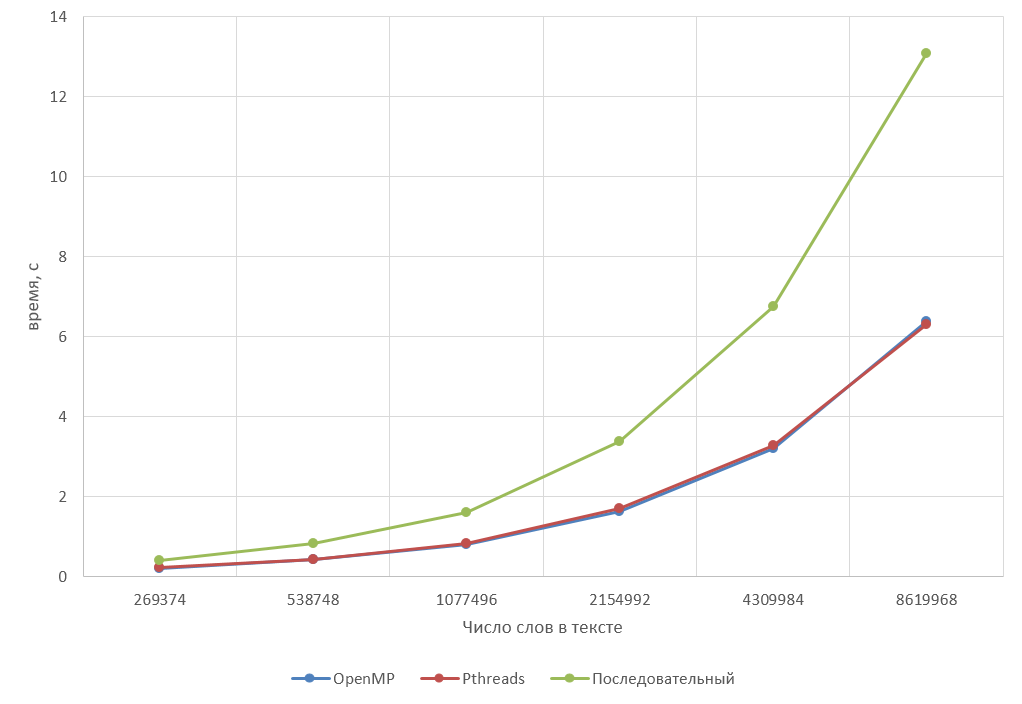
\includegraphics[width=\textwidth]{1}
	\caption{Зависимость времени от числа слов в тексте}
	\label{pic:wordchange}
\end{figure}

Из эксперимента видно, что параллельные решения работают приблизительно в два раза быстрее, чем последовательное решение. По скорости выполнения задачи параллельные решения в целом показывали близкие друг к другу результаты.

\subsection{Эксперимент 2}

\textbf{Количество потоков}: 1 -- 128

\textbf{Количество слов в тексте}: 2154988

\begin{table}[H]
	\centering
	\begin{tabular}{|c|c|c|c|}
		\hline
		Число потоков & Последовательный & OpenMP & Pthreads \\ \hline
		1   & 3.345            & \textbf{3.210}   & 3.240     \\ \hline
		2   & -                & 2.125  & \textbf{2.062}    \\ \hline
		4   & -                & \textbf{1.547}  & 1.627    \\ \hline
		8   & -                & \textbf{1.619}  & 1.672    \\ \hline
		16  & -                & \textbf{1.720}   & 1.797    \\ \hline
		32  & -                & \textbf{1.872}  & 1.941    \\ \hline
		64  & -                & \textbf{2.069}  & 2.293    \\ \hline
		128 & -                & \textbf{2.543}  & 2.688    \\
		\hline
	\end{tabular}
	\caption{Зависимость от количества потоков}
	\label{tab:threadchange}
\end{table}

\begin{figure}[H]
	\centering
	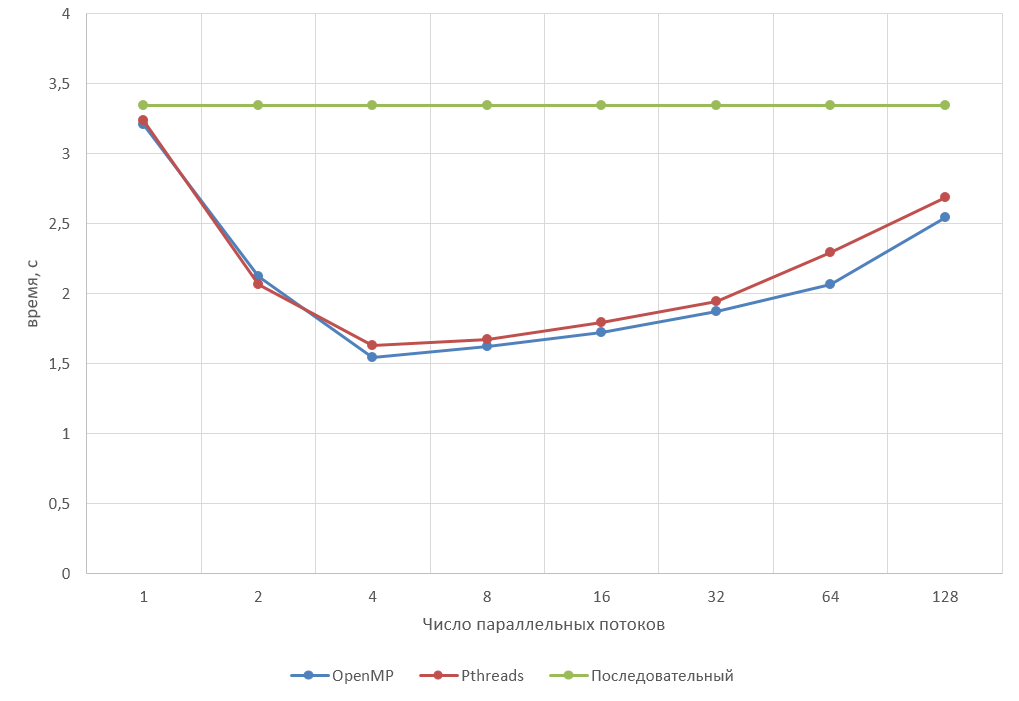
\includegraphics[width=\textwidth]{2}
	\caption{Зависимость от числа выделенных потоков}
	\label{pic:threadchange}
\end{figure}

Наилучшие показатели были получены при 4 потоках, прирост производительности при этом числе потоков составил:
\begin{itemize}
\item 54\% --- OpenMP;
\item 51\% --- Pthreads.
\end{itemize}

\subsection{Эксперимент 3}

В данном эксперименте проводится многократный запуск при одних и тех же характеристиках, для того чтобы вычислить:

\begin{itemize}
	\item математическое ожидание;
	\item дисперсию;
	\item доверительный интервал для оценки среднего,
\end{itemize}

что позволит более объективно оценить результаты алгоритмов.\\

\textbf{Количество потоков}: 4

\textbf{Количество слов в тексте}: 4309976

\begin{table}[H]
	\centering
	\begin{tabular}{|c|c|c|}
		\hline
		Последовательный & OpenMP & Pthreads \\ \hline
		6.465 & 3.089 & 3.126 \\ \hline
		6.522 & 3.081 & 3.144 \\ \hline
		6.471 & 3.063 & 3.132 \\ \hline
		6.602 & 3.142 & 3.122 \\ \hline
		6.516 & 3.045 & 3.143 \\ \hline
		6.441 & 3.076 & 3.273 \\ \hline
		7.529 & 3.152 & 3.377 \\ \hline
		6.666 & 3.151 & 3.239 \\ \hline
		6.632 & 3.123 & 3.203 \\ \hline
		6.882 & 3.362 & 3.145 \\
		\hline
	\end{tabular}
	\caption{Тестовая выборка для анализа}
	\label{tab:testvalues}
\end{table}

\begin{table}[H]
	\centering
	\begin{tabular}{|M{4.5cm}|M{4cm}|M{3.5cm}|M{3.5cm}|}
		\hline
		Характеристика         & Последовательный & OpenMP      & Pthreads    \\ \hline
		Среднее значение       & 6.6726           & 3.1284      & 3.1904      \\ \hline
		Дисперсия              & 0.00451584       & 0.00047524  & 0.000378951 \\ \hline
		Доверительный интервал (P = 0.95) & [6.469278635 - 6.669349082]      & [3.072340462 - 3.127503661] & [3.138601712 - 3.189571794] \\
		\hline
	\end{tabular}
	\caption{Вероятностные характеристики}
	\label{tab:stats}
\end{table}

Как видно из представленных характеристик, \textbf{OpenMP} является лучшим решением. Средняя скорость выполнения с его использованием немного выше, чем у pthreads.

\clearpage
\addcontentsline{toc}{section}{Вывод}
\section*{Вывод}
В данной работе были рассмотрены методы организации параллельных вычислений в программах с использованием OpenMP и pthreads.

Реализация на OpenMP проще и занимает меньшее количество строк кода по сравнению с pthreads. Например, в pthreads необходимо использовать функцию pthread\_join для синхронизации потоков, в то время как в OpenMP это контролируется самим фреймворком. Кроме того, функции, вызываемые при создании pthread, должны передавать аргументы через структуру, когда в случае с OpenMP это необязательно.

Эксперименты показали, что наилучшие результаты проиводительности на больших объемах текста можно получить на 4 потоках, где прирост производительности составляет 54\% для OpenMP и 51\% для pthreads. Скорее всего, данные результаты можно значительно улучшить, если реализовать более сложный алгоритм распараллеливания (например древовидную структуру распределения текста по потокам).

Отсюда можно сделать вывод, что организация параллельных вычислений программ имеет смысл в трудоемких задачах, хотя для тривиальных задач последовательное решение будет быстрее.
